\documentclass[dvipdfmx,autodetect-engine,titlepage]{jsarticle}
\usepackage[dvipdfm]{graphicx}
\usepackage{ascmac}
\usepackage{fancybox}
\usepackage{listings}
\usepackage{plistings}
\usepackage{itembkbx}
\usepackage{amsmath}
\usepackage{url}
\usepackage{graphics}
\usepackage{listings}
\usepackage{here}

\lstset{%
  language={C},
  basicstyle={\small},%
  identifierstyle={\small},%
  commentstyle={\small\itshape\color[rgb]{0,0.5,0}},%
  keywordstyle={\small\bfseries\color[rgb]{0,0,1}},%
  ndkeywordstyle={\small},%
  stringstyle={\small\ttfamily\color[rgb]{1,0,1}},
  frame={tb},
  breaklines=true,
  columns=[l]{fullflexible},%
  numbers=left,%
  xrightmargin=0zw,%
  xleftmargin=3zw,%
  numberstyle={\scriptsize},%
  stepnumber=1,
  numbersep=1zw,%
  lineskip=-0.5ex%
}

\textheight=23cm
\renewcommand{\figurename}{図}
\renewcommand{\tablename}{表}
\newenvironment{code}
{\vspace{0.5zw}\VerbatimEnvironment  \begin{screen} 
\baselineskip=1.0\normalbaselineskip
 \begin{Verbatim}}
{\end{Verbatim}
\baselineskip=\normalbaselineskip
 \end{screen}\vspace{0.5zw}} 

\title{セキュリティ・ネトワーク学実験3(B2)\\
Cプログラム脆弱性実習レポート\\
}
\author{26002000872\\Oku Wakana\\奥 若菜}
\date{Jun. 17 2022}

\begin{document}

\maketitle

\section*{問1}test.cをコンパイルして実行し、適当な短い英文字列Wakanaを入力して、表示を確かめた。下の図1は表示の様子をキャプチャしたものである。
入力した英文字列と同じようにWakanaと出力されることが確認できた。\\\\

\begin{figure}[H]
  \centering
  \fbox{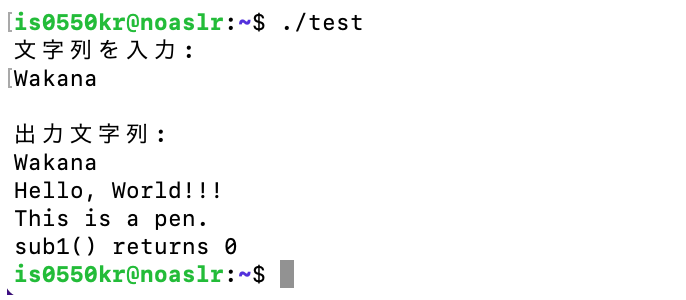
\includegraphics[scale=0.7]{f1.png} }
  \caption{}\label{fig:図1}
\end{figure}

\section*{問2}
\subsection*{2.1}
入力として文字列「\%E7\%AB\%8B\%E5\%91\%BD\%E9\%A4\%A8」を与えたとき、どのような文字列が表示されるかを確かめた。下の図2は表示の様子をキャプチャしたものであり、「立命館」と出力されることが確認できた。
入力した文字列がそのまま表示されない理由として、まずbufに入力された\%xxという形式の部分は、xxを16進数とみなして1バイトの値に置き換えられ、bufに上書きされる処理がプログラム中でなされる。そして、
bufに格納されたバイナリデータは、一定の規則に基づいて、テキストデータにエンコードされ、出力されるためである。入出力の関係から、文字コードの方式にはUTF-8が使用されていることが分かった。\\\\

\begin{figure}[H]
  \centering
  \fbox{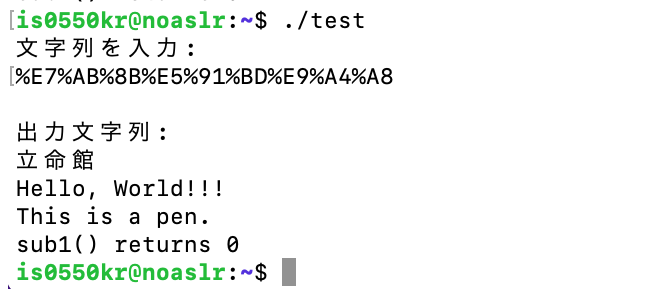
\includegraphics[scale=0.7]{f2.png} }
  \caption{}\label{fig:図2}
\end{figure}

\subsection*{2.2}
2.1章で明らかになったことを考慮して入力を行い、レポート作成者の名前である「奥若菜」を1行目に出力した。下の図3は表示の様子をキャプチャしたものであり、UTF-8の文字コードを\%xxの形式で入力することにより、目的の文字列が表示されたことが確認できる。\\

\begin{figure}[H]
  \centering
  \fbox{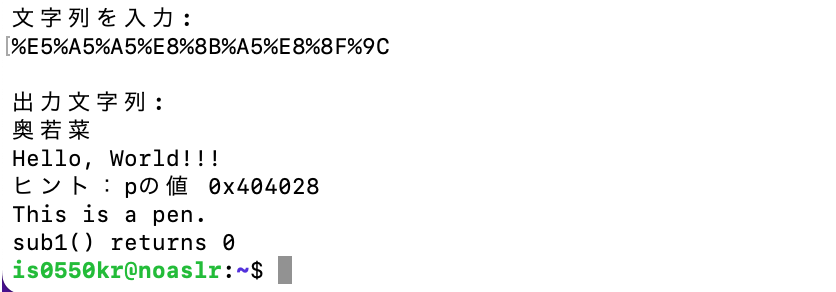
\includegraphics[scale=0.7]{f3.png} }
  \caption{}\label{fig:図3}
\end{figure}

\section*{問3}
入力として適当な文字を与え、配列変数strの中身を強制的に書き換えることによって、出力の2行目がHello, World!!!ではなく、Ritsumeikanとなるようにする。
文字列の入出力は関数sub1で行われ、1行目と2行目には、sub1のローカル変数であるbufとstrがそれぞれ表示される。下の図4は、グローバル変数とsub1の各変数が格納されているアドレスを表示したものである。
プログラム中で、bufは32バイトの大きさで宣言されており、図4を見ると、bufの先頭アドレスは
0xbfffe5dcで、strの先頭アドレスは、そこから32バイト後ろにずらした0xbfffe5fcとなっていることが分かる。\\

\begin{figure}[H]
  \centering
  \fbox{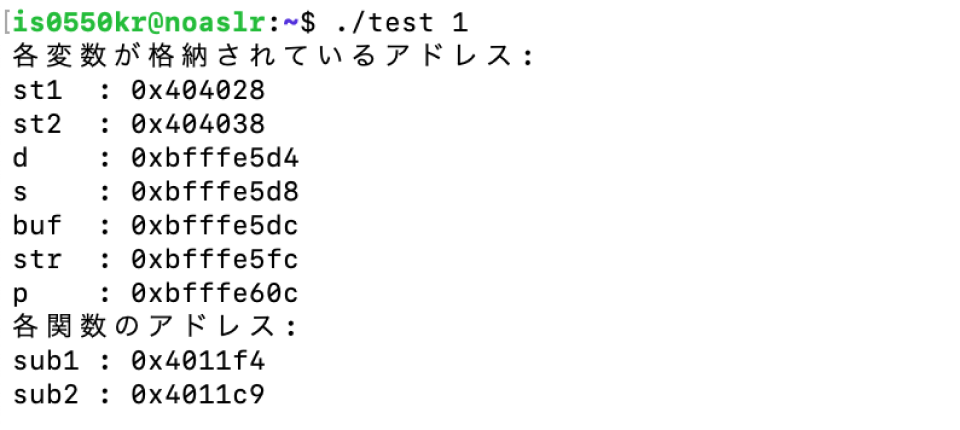
\includegraphics[scale=0.3]{o1.png} }
  \caption{各変数のアドレス}\label{fig:図10}
\end{figure}

bufの入力がgets()で行われることから、bufに32バイトより長い文字列を入力することによって、bufの領域の後ろに存在するstrの値を上書きすることができると考えた。
下の図5は、入力と表示の様子をキャプチャしたものである。wを32バイト分入力することにより、bufの領域を埋め、その後ろにRitsumeikanと入力することで、strの中身を書き換え、
結果2行目に
Ritsumeikanと表示させることができた。\\
\begin{figure}[H]
  \centering
  \fbox{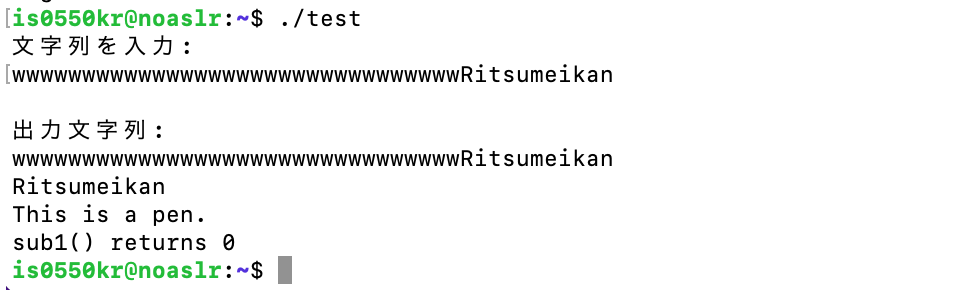
\includegraphics[scale=0.6]{f4.png} }
  \caption{}\label{fig:図4}
\end{figure}

\section*{問4}
入力として適当な文字を与え、出力の3行目がThis is a pen.ではなく、I have an apple.となるようにする。3行目には、ポインタ変数pが指すアドレスに格納されている値が出力される。また、プログラム中では、pにはst1のアドレスが格納される。よって、入力からpの値をst2のアドレスに書き換えることによって、st2に格納されているI have an apple.の文字列を表示させることができると考えた。
図5は、実行の様子をキャプチャしたものである。図5より、pが格納されているアドレスは、0xbfffe60cで、bufの先頭アドレスから48バイト後ろあることが分かる。そこで、まずbufとstrの領域を埋めるために、oを48バイト分入力し、その後ろにst2のアドレスを入力した。
このとき、 IntelのCPUはリトルエンディアンであることを考慮し、アドレスは4バイトずつ、下位バイトから順に入力した。
結果、3行目にst2の値であるI have an apple.の文字列を表示することができた。\\\\
\begin{figure}[H]
  \centering
  \fbox{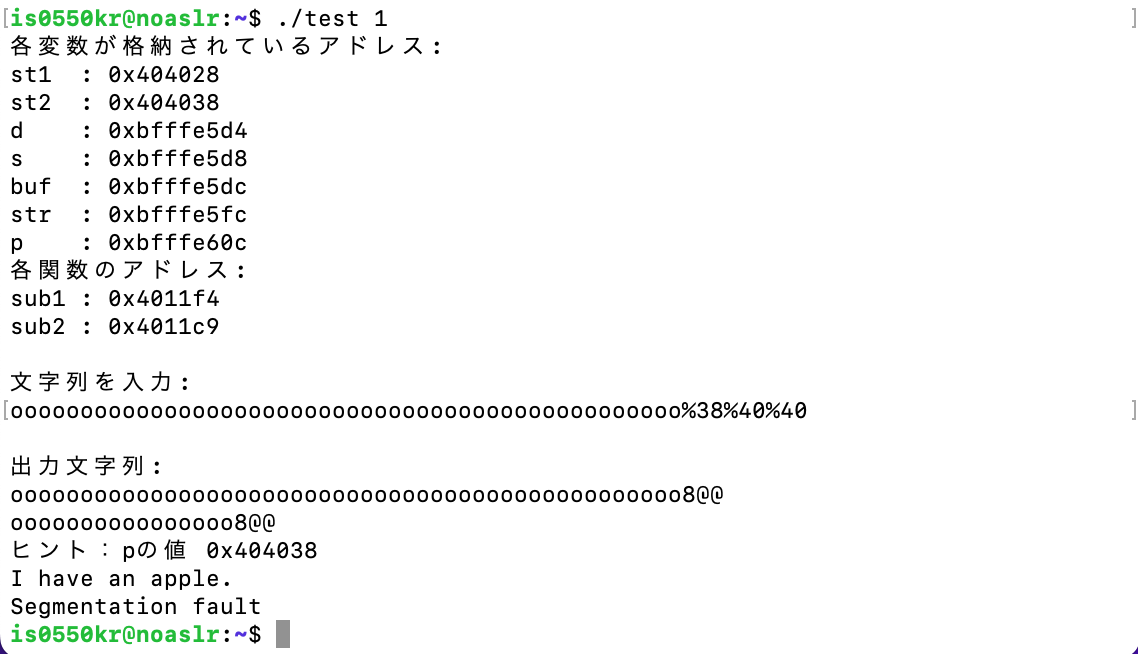
\includegraphics[scale=0.6]{f5.png} }
  \caption{}\label{fig:図5}
\end{figure}

\section*{問5}
関数sub1()からreturnするタイミングで関数sub2()を呼び出し、出力の4行目にBingo!と表示されるようにする。この問題では、プログラム内部を監視するためのデバッガとしてGdbを使用した。
まず、本来のsub1()からの戻りアドレスを知るために、disassembleコマンドを使用して、main関数のコードを逆アセンブルした。下の図7は表示されたマシン命令の内容である。青い部分がsub1を呼び出す命令なので、その一行下のアドレス0x004014bcが
sub1の戻りアドレスである。
\begin{figure}[H]
  \centering
  \fbox{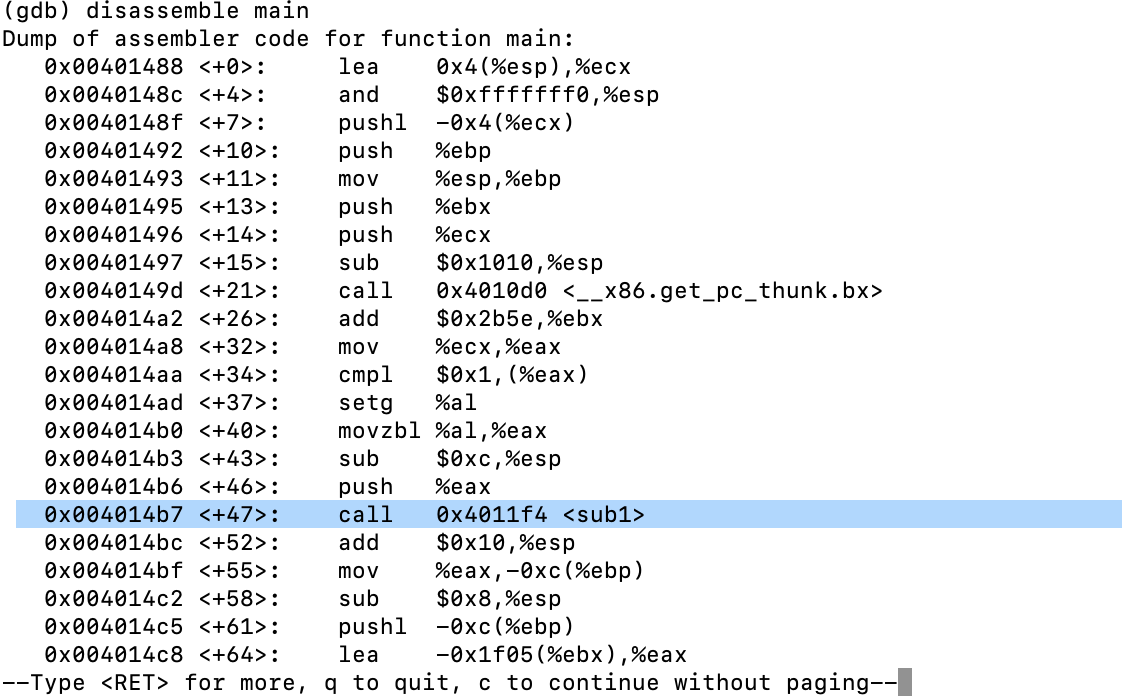
\includegraphics[scale=0.6]{o3.png} }
  \caption{main関数のマシン命令}\label{fig:図11}
\end{figure}

次に、入力を受け取る直前において、bufの先頭アドレスから108バイト分のメモリに、それぞれどのような値が格納されているかを表示させた。
図8において、青い部分はbuf以降のsub1のローカル変数が格納されている範囲である。上から4行(32バイト)はbufの領域であり、まだ何も格納されていない。また、その下の2行(16バイト)はstrの領域であり、Hello, World!!!の文字列がバイナリで格納されている。さらに1つ下の行の先頭から4バイトはpの領域であり、st1のアドレスである0x404028がリトルエンディアンで格納されている。
\begin{figure}[H]
  \centering
  \fbox{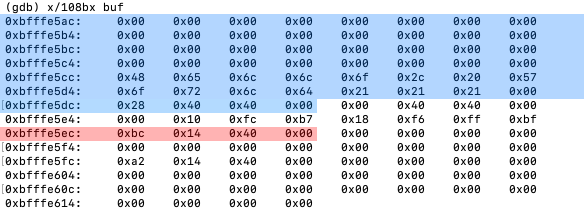
\includegraphics[scale=0.6]{o4.png} }
  \caption{bufを先頭にしたメモリ}\label{fig:図12}
\end{figure}

ローカル変数の領域の後ろに、戻りアドレスの0x004014が格納されている場所がないか探したところ、図8の赤い部分に格納されていることが確認できた。よって、戻りアドレスが格納されている0xbffffe5ecからの4バイトを書き換えることで、sub1がreturnするタイミングで、sub2を呼び出せるはずである。\\\\
しかし、bufに64バイトの文字列とsub2のアドレスを入力したところ、プログラムが動作しなくなってしまった。これは、ローカル変数の領域(青い部分)と戻り値の領域(赤い部分)の間に存在する、レジスタの領域を書き換えてしまったためだと考えられる。下の図9はi fコマンドで各レジスタのアドレスを表示した結果である。今回書き換えた戻り値アドレスが格納されている領域の前にレジスタ領域が存在することが分かる。\\
\begin{figure}[H]
  \centering
  \fbox{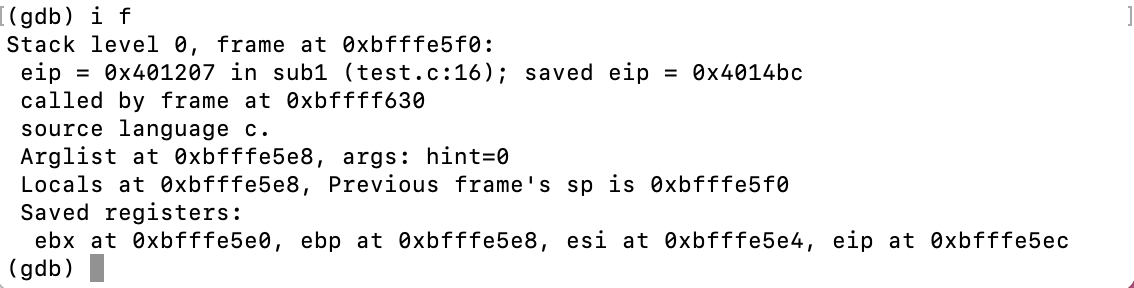
\includegraphics[scale=0.6]{o6.png} }
  \caption{各レジスタのアドレス}\label{fig:図13}
\end{figure}

また、ポインタ変数pの値を書き換えることも、Segmentation faultを起こし、プログラムを中断させる原因になる。以上のことに注意して、メモリの書き換えが行われないように入力したものが下の図10である。sub2を呼び出し、出力の4行目にBingo!と表示させることができた。\\
\begin{figure}[H]
  \centering
  \fbox{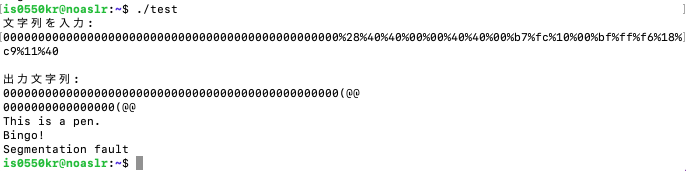
\includegraphics[scale=0.5]{f6.png} }
  \caption{出力結果}\label{fig:図14}
\end{figure}
\end{document}